%!TEX program = xelatex
\documentclass{beamer}
\usepackage[russian]{babel}
\usepackage{blindtext}

\usepackage{media9}

\usetheme{Execushares}

\title{Анализ качества восстановления каплинга в обратной задаче Курамото-модели для различных модельных функций}
\subtitle{Научный семинар}
\author{Антон Савостьянов}
\date{17 ноября, 2017}

\setcounter{showSlideNumbers}{1}

\begin{document}
	\setcounter{showProgressBar}{0}
	\setcounter{showSlideNumbers}{0}

	\frame{\titlepage}

	\begin{frame}
		\frametitle{Contents}
		\begin{enumerate}
			\item Модель Курамото \\ \textcolor{ExecusharesGrey}{\footnotesize\hspace{1em} Постановка задачи и обозначения}
			\item Кусочно-константные модельные приближения $k_0(t)$ \\ \textcolor{ExecusharesGrey}{\footnotesize\hspace{1em} 
			%\begin{enumerate}
				Положительный и отрицательный шоки $k_0(t)$; случай нарушения основного Курамото-неравенства
			%\end{enumerate}
			}
			\item Приближение $k_0(t)$ простыми колебаниям ($\sin(t)$) \\ \textcolor{ExecusharesGrey}{\footnotesize\hspace{1em} Влияние спектральных параметров на качество восстановления}
			\item Авторегрессионный процесс как $k_0(t)$ \\ \textcolor{ExecusharesGrey}{\footnotesize\hspace{1em} Слабая стационарность; влияение параметров на среднее качество восстановления; средняя доля катастроф}
			\item Итоги
		\end{enumerate}
	\end{frame}

	\setcounter{framenumber}{0}
	\setcounter{showProgressBar}{1}
	\setcounter{showSlideNumbers}{1}
	
\begin{frame}
	\frametitle{Модель Курамото}
	\begin{itemize}
		\item Модель предложена в 1975 \textit{Yoshiki Kuramoto}
		\item Поведение осцилляторов в модели:
		\[
		X_i(t)=a_i(t)\sin\left( \Omega_i t + \varphi_i \right)
		\]
		\[
		X_i(t)=\sin\left(\theta_i(t)\right)
		\]
		\item Явление синхронизации: $\Omega_i=\Omega_j=\Omega$ (\textbf{частотная}) и $\varphi_i-\varphi_j=const$ (\textbf{фазовая})
		\begin{multline*}
		\varphi_i-\varphi_j=\left( \Omega t + \varphi_i \right)-\left( \Omega t + \varphi_j \right)=\theta_i(t)-\theta_j(t) \Rightarrow \\
		\Rightarrow \dot{\theta_i}-\dot{\theta_j}=0
		\end{multline*}
	\end{itemize}
\end{frame}

\begin{frame}
\frametitle{Модель Курамото}
\begin{itemize}
	\item Динамика фаз осцилляторов:
	\[
	\dot{\theta_i} = \omega_i +\sum_{j=1}^n \frac{k_{ij}}{2}(t)\sin\left(\theta_j-\theta_i\right),
	\]
	где $\omega_i$ --- разница фаз, $k_{ij}(t)$ --- каплинг осцилляторов, а $\theta_i-\theta_j$ --- фазовая разница.
	\item Положим задачу для двух осцилляторов ($i,j=1,2$) с постоянными естественными частотами ($\omega_i=const$) и симметричным каплингом ($k_{12}(t)=k_{21}(t)=k(t)$). Вычитая уравнения ($\Delta\omega=\frac{\omega_1-\omega_2}{2}$, $\theta_1-\theta_2=\theta$):
	\[
		\dot{\theta}=2\Delta \omega - k(t)\sin \theta(t)
	\]
	\item \textbf{Обратная задача:} по $X(t)$ и $Y(t)$ восстановить $k(t)$
\end{itemize}
\end{frame}

\begin{frame}
\frametitle{Обратная задача}
\begin{alertblock}{Задача}
	Оценить качество восстановления на модельных функциях, после чего использовать полученные результаты для анализа качества восстановления на реальных данных.
\end{alertblock}
\begin{exampleblock}{Процедура восстановления}
\begin{enumerate}
	\item Выберем некоторое начальное приближение каплинга $k_0(t)$; решим дифференциальное уравнение $\dot{\theta}=2\Delta \omega - k_0(t)\sin \theta(t)$;
	\item Введем два виртуальных маятника: $X_0=\sin(\Omega t+\theta(t))$, $Y_0=\sin(\Omega t)$, посчитаем их скользящую корреляцию в окне периода $C_0(t)$;
	\item Исходя из предположений квазистационарности ($\dot{\theta} \approx 0$): $\varphi_0=\arccos C_0(t) \Rightarrow \hat{k}(t)=\frac{2\Delta \omega}{\sin\varphi_0}$
\end{enumerate}
\end{exampleblock}
\end{frame}

\begin{frame}
\frametitle{Кусочно-константные $k_0(t)$}
Пусть
\[
k_0(t)=\begin{cases}
d, \; 0 \le t \le 2T \wedge t \ge 2T+\tau \\
d+\Delta d, \; 2T \le t \le 2T+\tau
\end{cases}
\]
\begin{itemize}
	\item $d$ --- невозмущенное значение;
	\item $\Delta d$ --- величина возмущения (шока);
	\item $\tau$ --- длительность возмущения (шока);
	\item $T$ --- общий главный период маятников.
\end{itemize}

Заметим, что если $\Delta d < 0$, то может быть нарушено основное Курамото-неравенство:
\[
\left|\frac{2\Delta\omega}{k_0(t)}\right|\le 1
\]
\end{frame}

\begin{frame}
\frametitle{Кусочно-константные $k_0(t)$ ($\Delta d >0$)}
\phantom{123}   
\begin{center}
	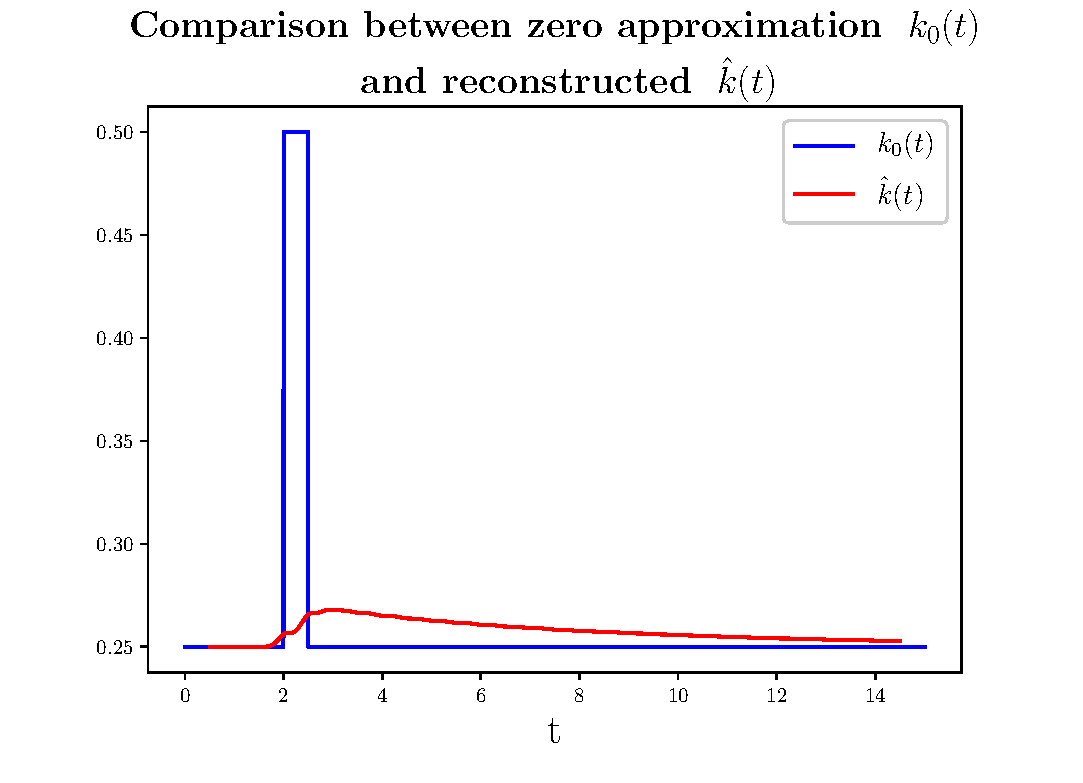
\includegraphics[width=0.45\textwidth]{2206_khat_positive_15.eps} %
	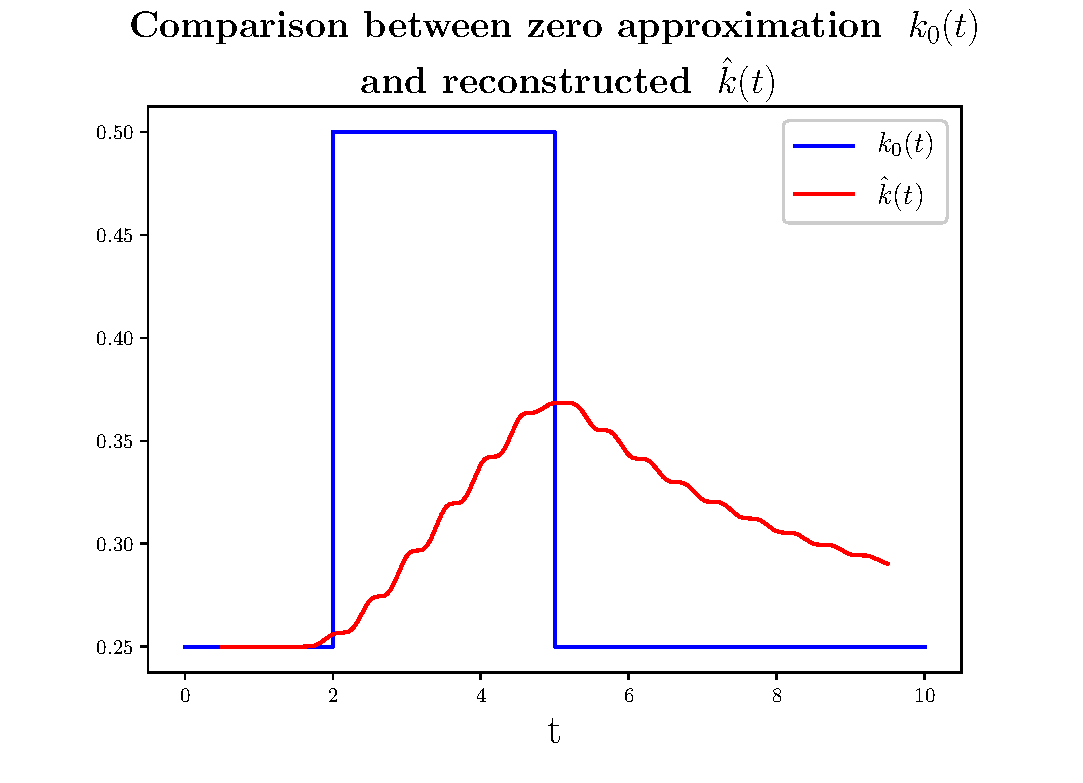
\includegraphics[width=0.45\textwidth]{2206_khat_positive_long_10.eps}
	\vfill
	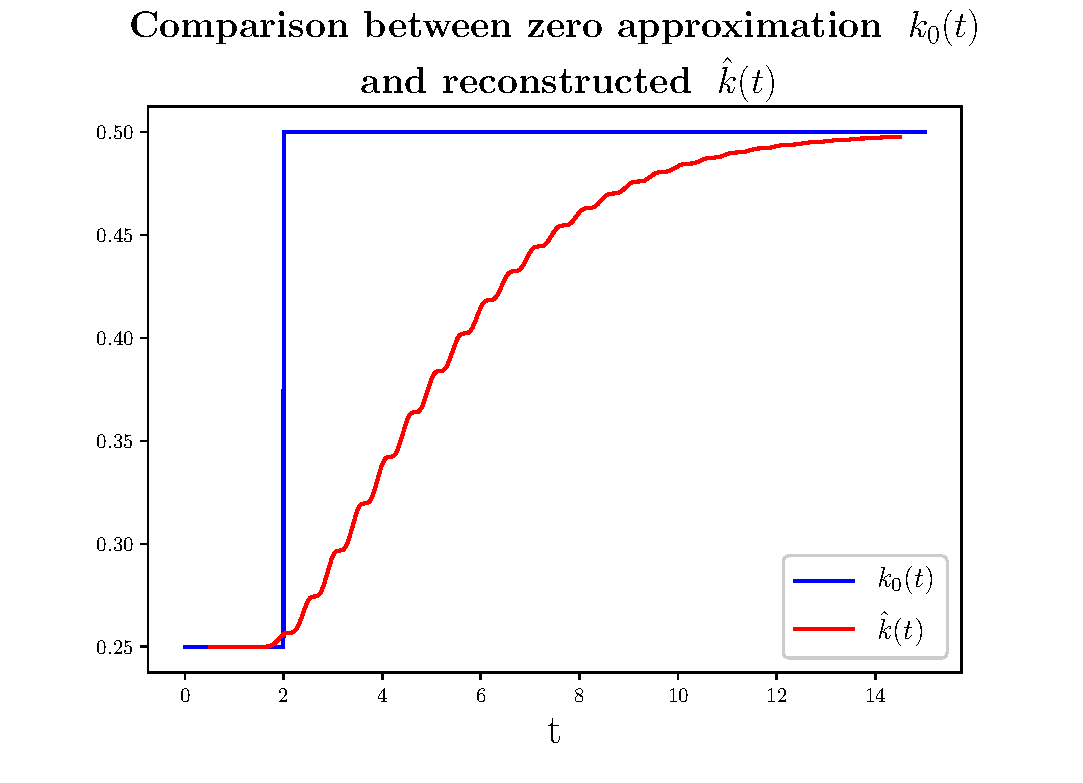
\includegraphics[width=0.45\textwidth]{2206_khat_positive_end_15.eps}
\end{center}
\end{frame}

\begin{frame}
\frametitle{Меры качества восстановления}
Для данного случая будем рассматривать следующие метрики для сравнения $k_0(t)$ и $\hat{k}(t)$:
\begin{enumerate}
	\item $jumpK=\frac{\left| \hat{k}(2T+\tau)-d \right|}{\Delta d}$
	\item $jumpKC=\frac{\max\limits_{t\ge 2T+\tau} \left| \hat{k}(t)-d \right|}{\Delta d}$
	\item $jumpKR=\frac{1}{nT}\sqrt{\int_0^{nT} \left(\hat{k}(t)-k_0(t)\right)^2 dt}$
	\item $jumpKR_0=\frac{1}{n\sigma(k_0(t))T}\sqrt{\int_0^{nT} \left(\hat{k}(t)-k_0(t)\right)^2 dt}$
\end{enumerate}
\end{frame}

\begin{frame}
\frametitle{Кусочно-константные $k_0(t)$ ($\Delta d >0$)}
\phantom{123}   
\begin{center}
	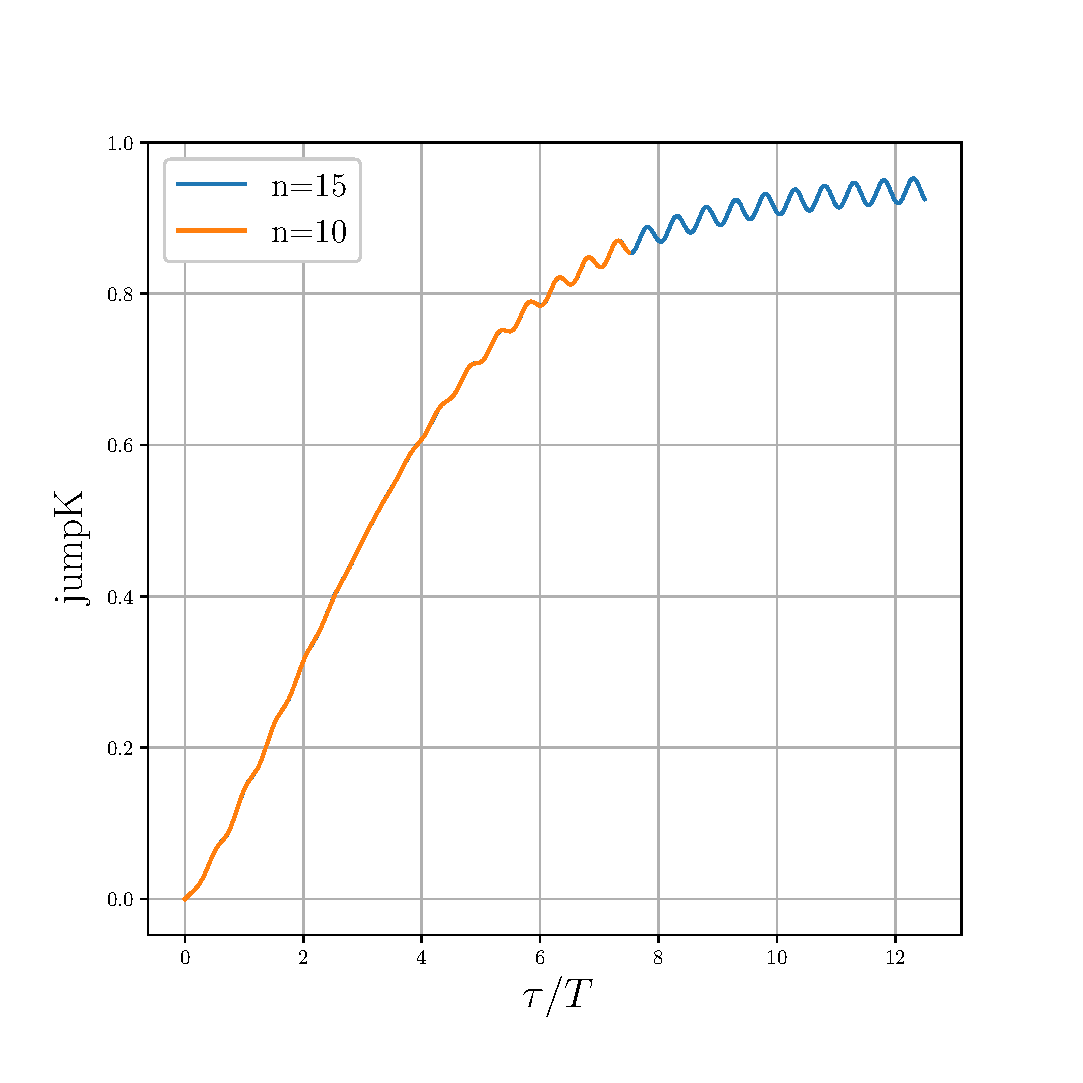
\includegraphics[width=0.37\textwidth]{2206_k-10-15.eps} %
	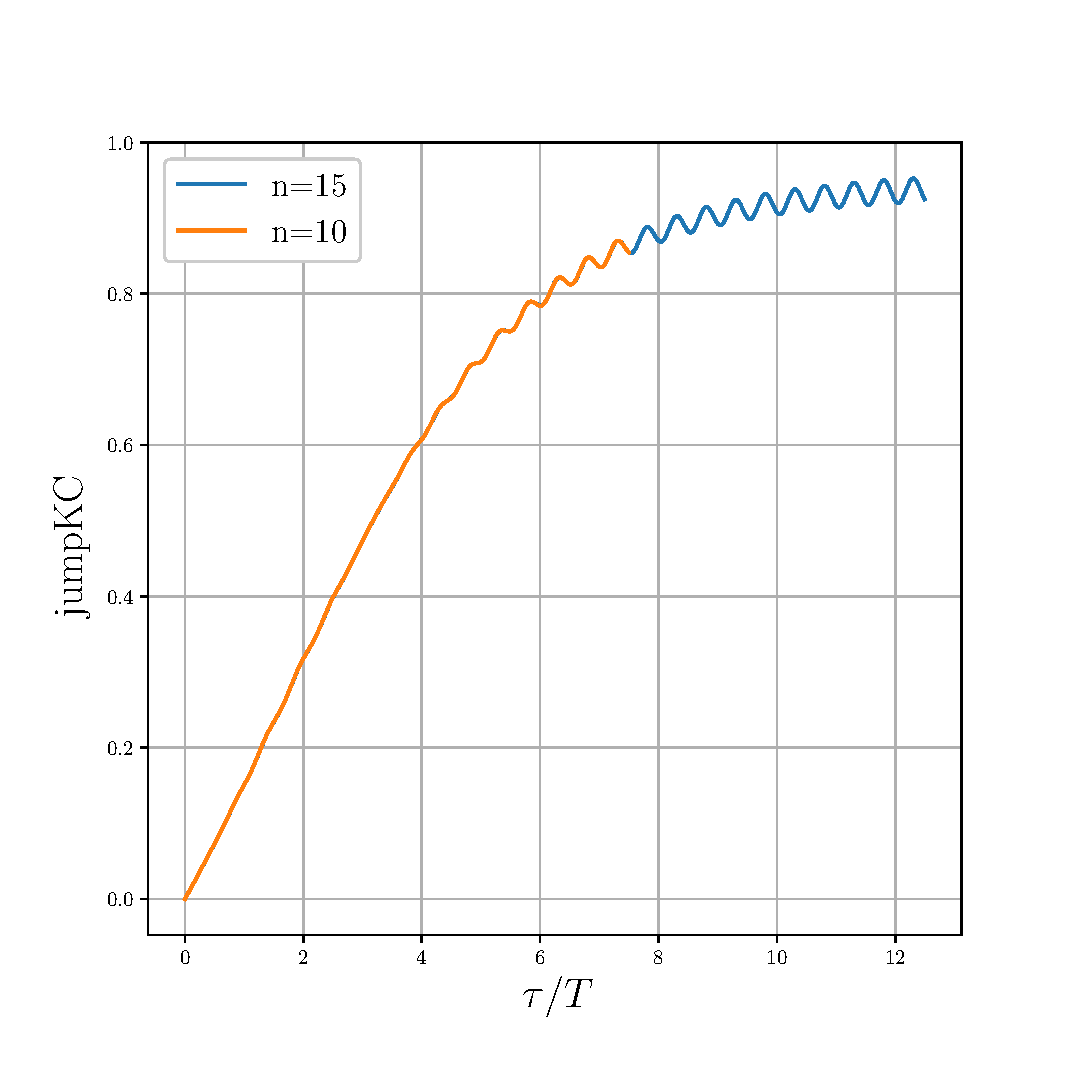
\includegraphics[width=0.37\textwidth]{2206_kC-10-15.eps}
	\vfill
	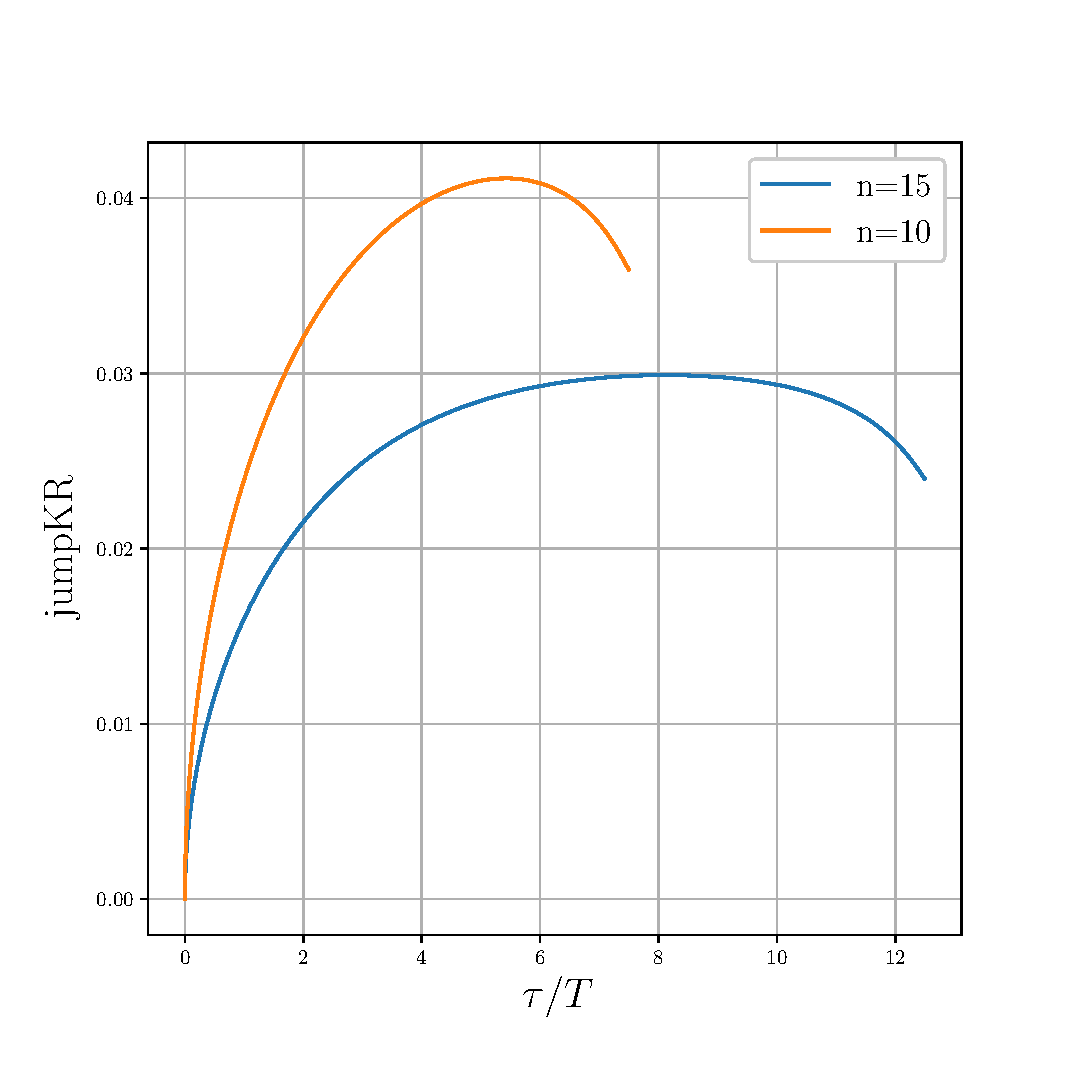
\includegraphics[width=0.37\textwidth]{2206_kR-10-15.eps} %
	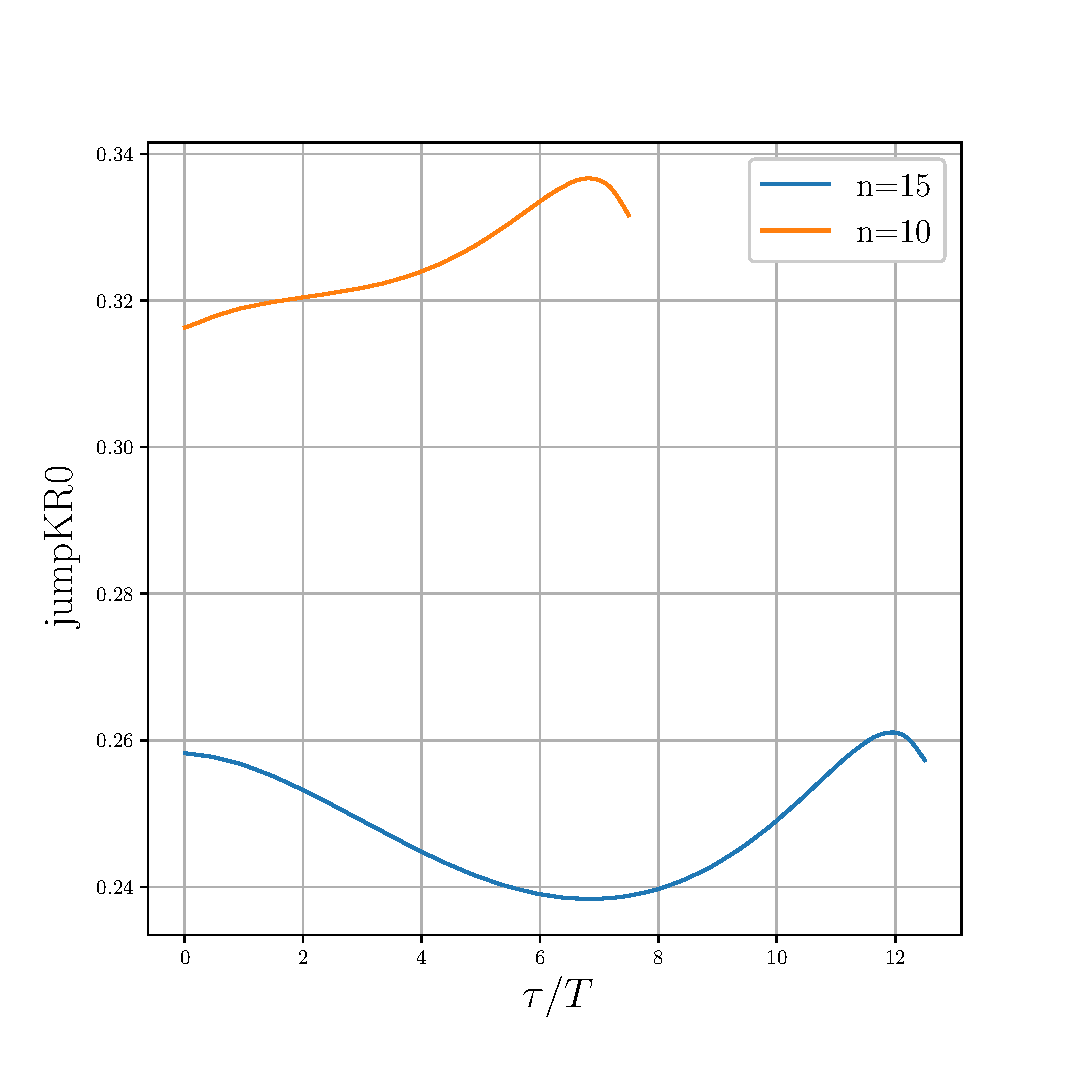
\includegraphics[width=0.37\textwidth]{2206_kR0-10-15.eps}
\end{center}
\end{frame}

\begin{frame}
\frametitle{Кусочно-константные $k_0(t)$ ($\Delta d <0$)}
\phantom{123}   
\begin{center}
	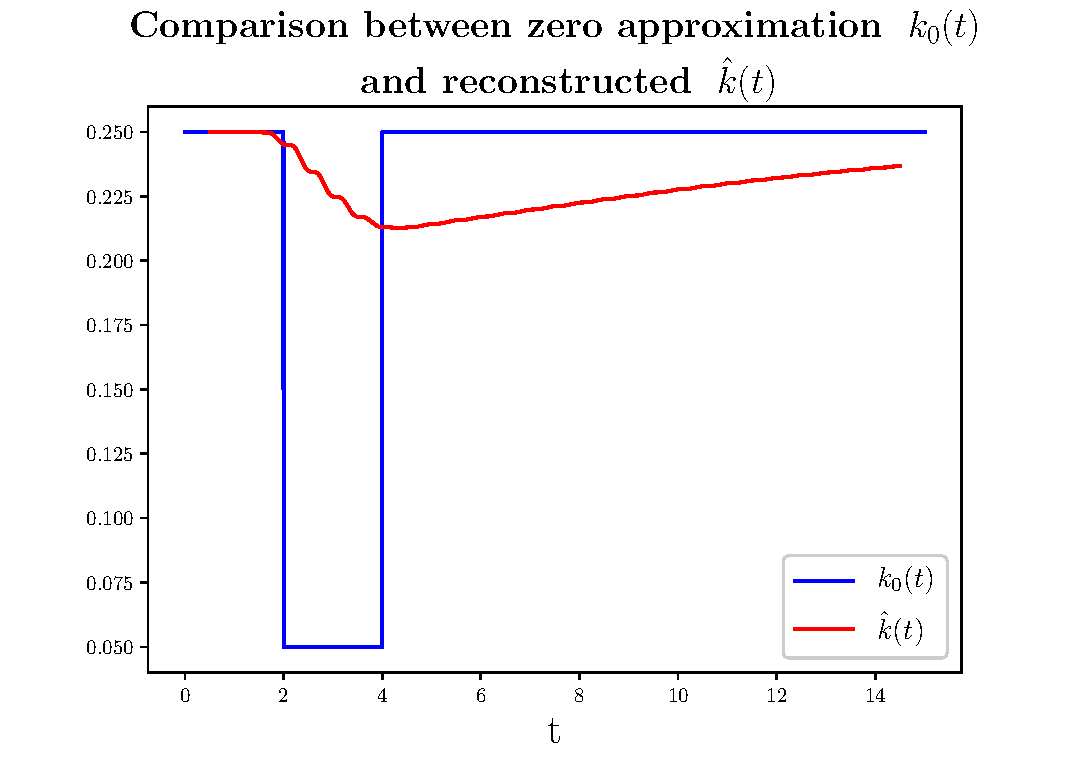
\includegraphics[width=0.45\textwidth]{2306_khat_neg_800_15.eps} %
	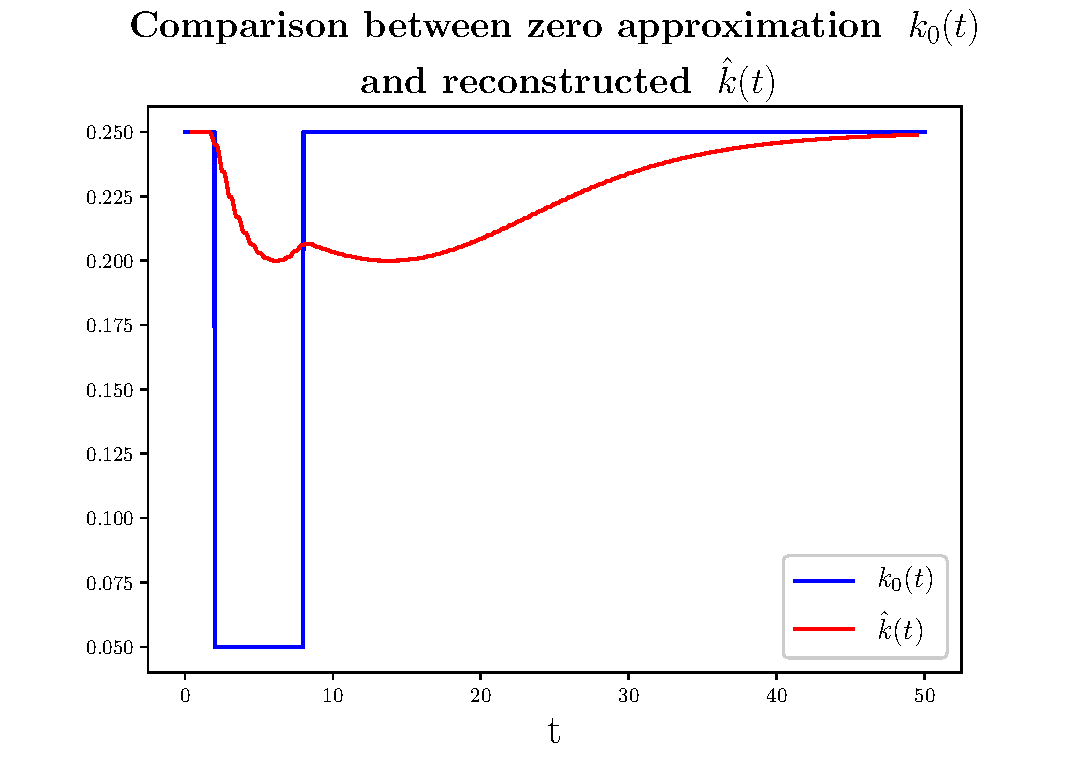
\includegraphics[width=0.45\textwidth]{2306_khat_neg_2400_50.eps}
	\vfill
	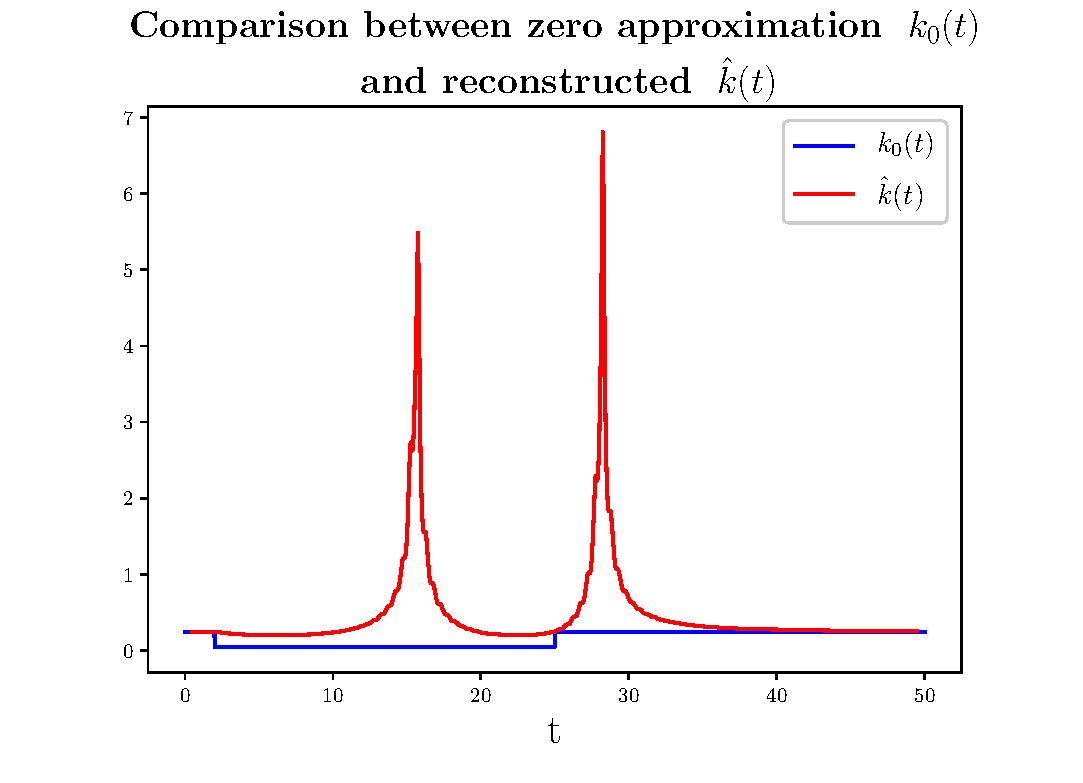
\includegraphics[width=0.45\textwidth]{2306_khat_neg_9200_50.eps}
\end{center}
\end{frame}

\begin{frame}
\frametitle{Кусочно-константные $k_0(t)$ ($\Delta d <0$)}
\begin{itemize}
	\item Пожалуйста, включите видео \texttt{const\_anim.mp4}
	\item Можно заметить две характерных длительности шока, нарушающего основное Курамото-неравенство: момент появления второго экстремума и момент появления сингулярности (катастрофы)
\end{itemize}
\end{frame}

\begin{frame}
\frametitle{Кусочно-константные $k_0(t)$ ($\Delta d <0$)}
\phantom{123} 
Приведем два графика времени появлений второго экстремума и катастрофы: для слабого ($d=0.25, \Delta d=-0.2$) и сильного ($d=2.5, \Delta d=-2.45$) каплингов
\begin{center}
	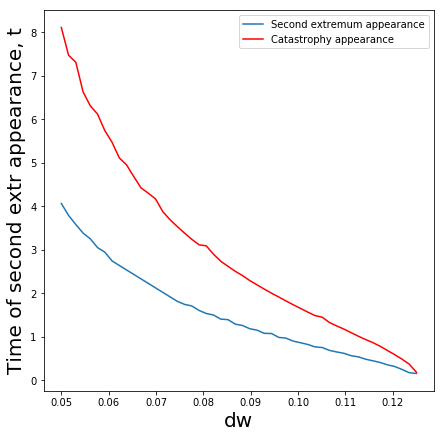
\includegraphics[width=0.45\textwidth]{1711_extr_weak.png} %
	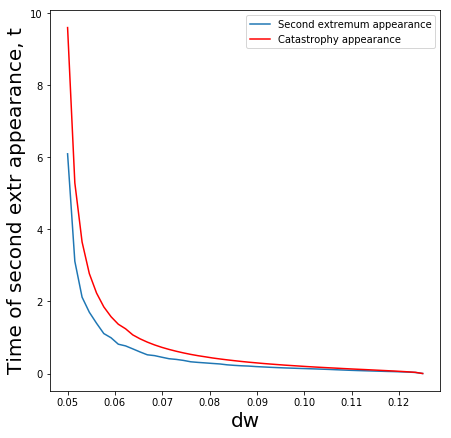
\includegraphics[width=0.45\textwidth]{1711_extr_strong.png}
\end{center}
\end{frame}

\begin{frame}
\frametitle{Приближение $k_0(t)$ синусом}
\begin{minipage}{3cm}
	\[
	k_0(t)=A\sin(Bt+\varepsilon)+C,
	\]
	$A$ --- амплитуда, \\ $B$ --- частота, $C$ --- среднее значение
	$C-A \le 2\Delta \omega $
\end{minipage}
\begin{minipage}{7cm}
	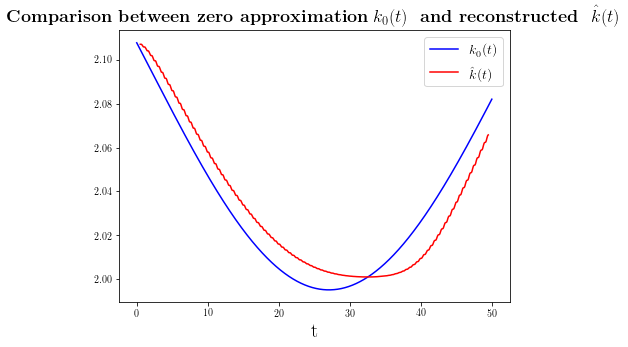
\includegraphics[height=4cm]{download.png}
\end{minipage}

\begin{center}
Пожалуйста, включите видео \texttt{sink\_anim.mp4}	
\end{center}
\end{frame}

\begin{frame}
\frametitle{Приближение $k_0(t)$ синусом ($jumpRK_0$)}
Приведем графики качества восстановления $jumpRK_0$ при различных $C$:
\begin{center}
	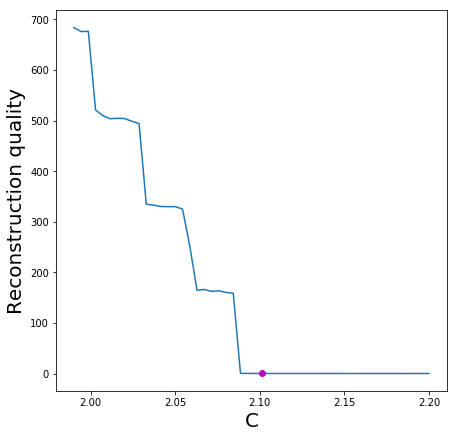
\includegraphics[width=0.45\textwidth]{sinC1.png} %
	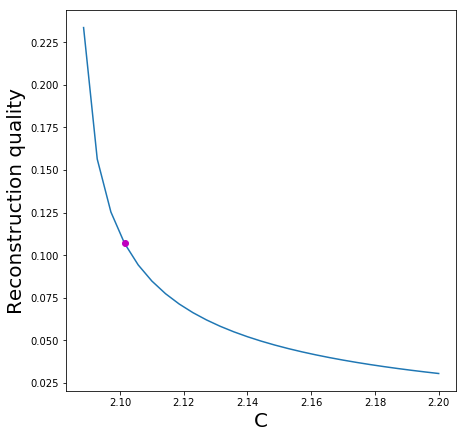
\includegraphics[width=0.45\textwidth]{sinC2.png}
\end{center}
\end{frame}

\begin{frame}
\frametitle{Приближение $k_0(t)$ синусом ($jumpRK_0$)}
Приведем графики качества восстановления $jumpRK_0$ при различных $B$: слева амплитуда не позволяет нарушений Курамото-неравенства, а справа позволяет (ось ординат логарифмическая):
\begin{center}
	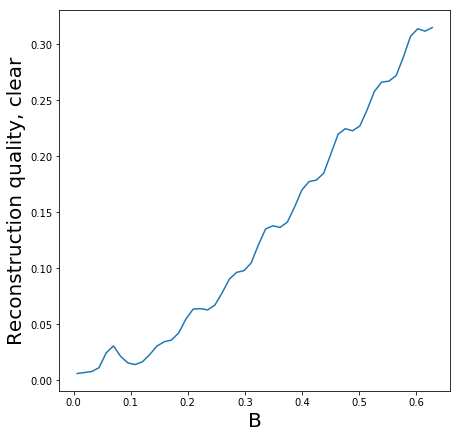
\includegraphics[width=0.45\textwidth]{sinB1.png} %
	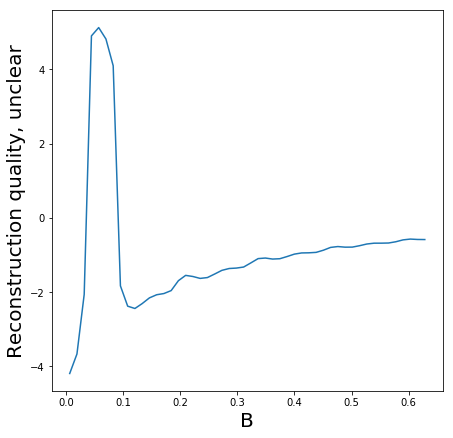
\includegraphics[width=0.45\textwidth]{sinB2.png}
\end{center}
\end{frame}

\begin{frame}
	\frametitle{$k_0(t)$ как реализация AR(1)}
	\begin{itemize}
		\item 	Положим $k_0(t)$ следующим случайным процессом:
		\[
		k_0(t)=\alpha k_0(t-1)+m+\xi(t-1),\;\xi(t)\sim N(0, \sigma^2)
		\]
		Такой процесс называется \textbf{авторегрессионным}.
		\item Через характерное время $\tau=\frac{1}{1-\alpha}$ процесс становится стационарным в слабом смысле, причем:
		\[\mathbb{E}[k_0]=\frac{m}{1-\alpha}\]
		\[
		\sigma[k_0]=\frac{\sigma}{\sqrt{1-\alpha^2}}
		\]
	\end{itemize}
\end{frame}

\begin{frame}
\frametitle{$k_0(t)$ как реализация AR(1)}
\phantom{123}
\begin{center}
	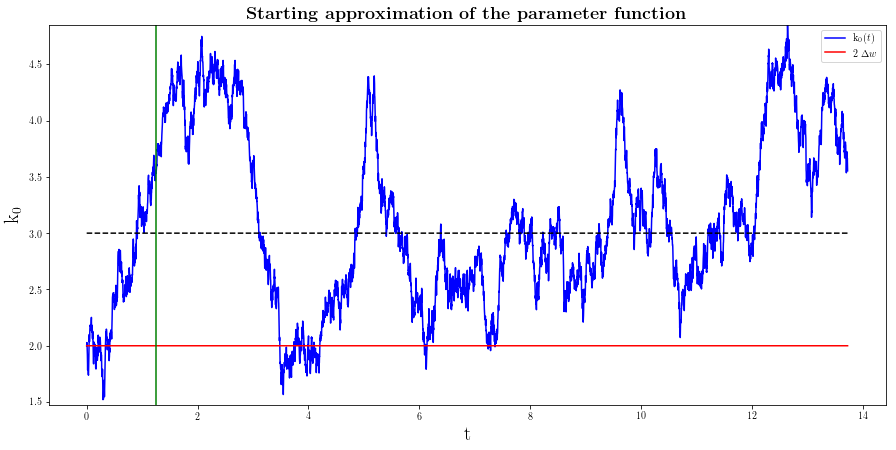
\includegraphics[width=0.7\textwidth]{stk1.png} 
	
	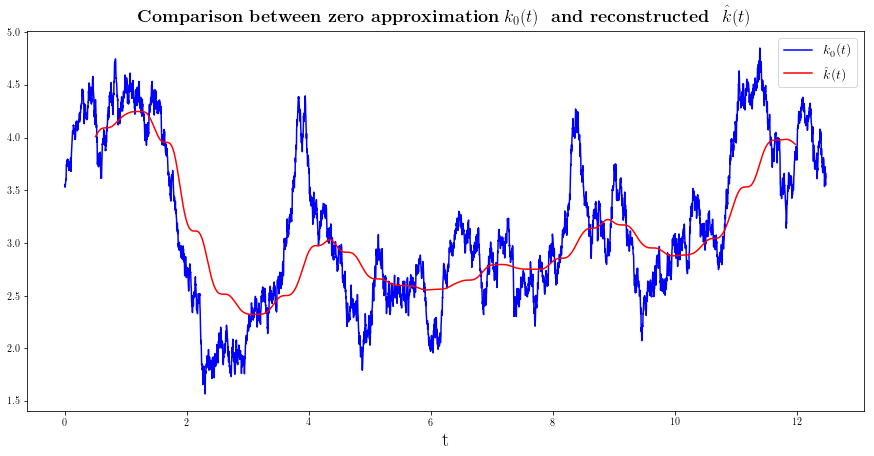
\includegraphics[width=0.7\textwidth]{stk1-1.png}
\end{center}
\end{frame}

\begin{frame}
\frametitle{$k_0(t)$ как реализация AR(1)}
\phantom{123}
\begin{center}
	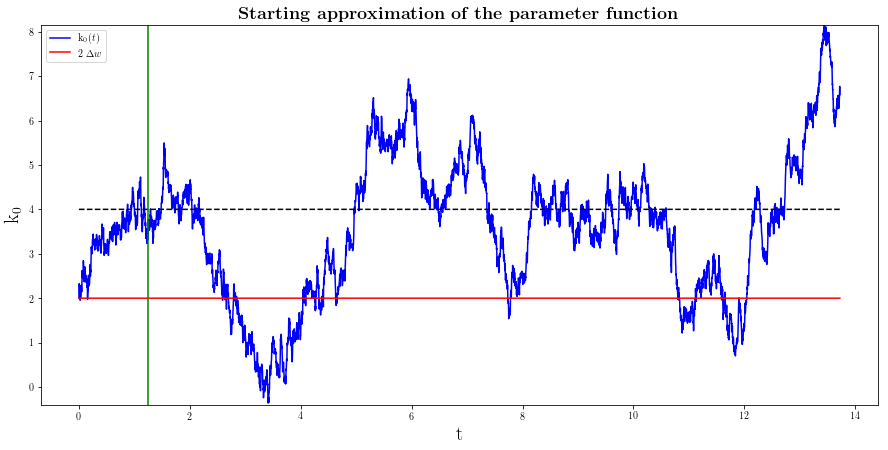
\includegraphics[width=0.7\textwidth]{stk2.png} 
	
	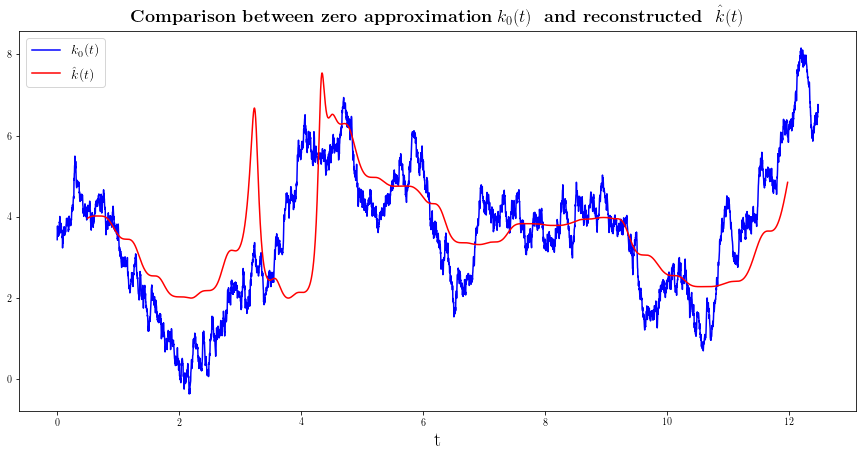
\includegraphics[width=0.7\textwidth]{stk2-1.png}
\end{center}
\end{frame}

\begin{frame}
\frametitle{$k_0(t)$ как реализация AR(1)}
\phantom{123}
\begin{center}
	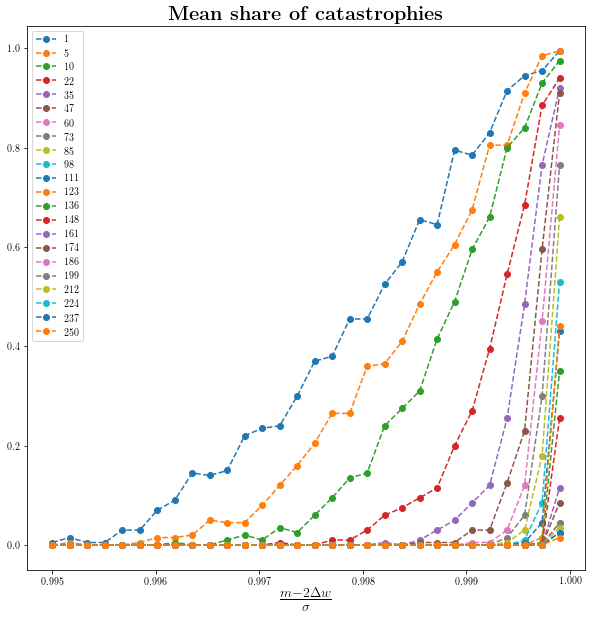
\includegraphics[width=0.7\textwidth]{sh1.png}
\end{center}
\end{frame}

\begin{frame}
\frametitle{$k_0(t)$ как реализация AR(1)}
\phantom{123}
\begin{center}
	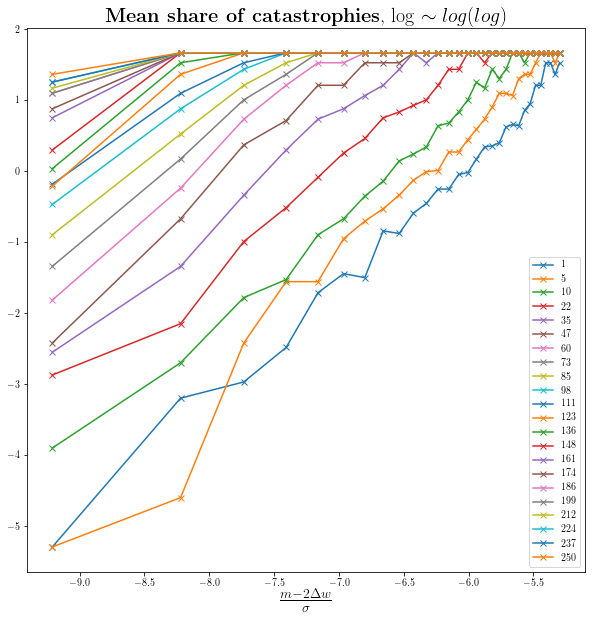
\includegraphics[width=0.45\textwidth]{sh2.png} 
	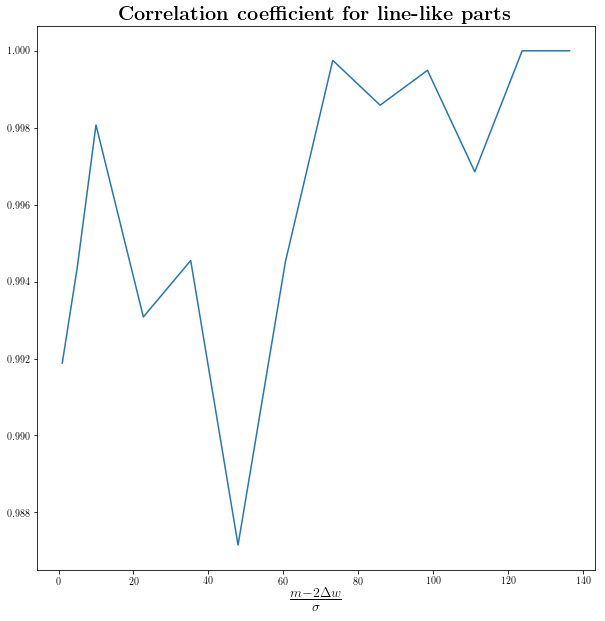
\includegraphics[width=0.45\textwidth]{sh3.png}
Таким образом доля катастроф есть $\approx f((1-\alpha))e^{-(1-\alpha)}$!
\end{center}

\end{frame}

\section{Спасибо за внимание!}

\begin{frame}
\frametitle{$k_0(t)$ как реализация AR(1)}
\phantom{123}
\begin{center}
	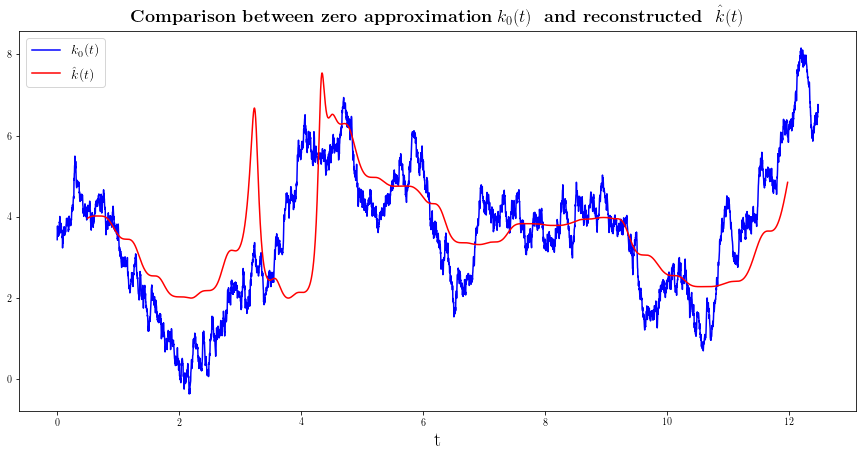
\includegraphics[width=0.7\textwidth]{stk2-1.png} 
	
	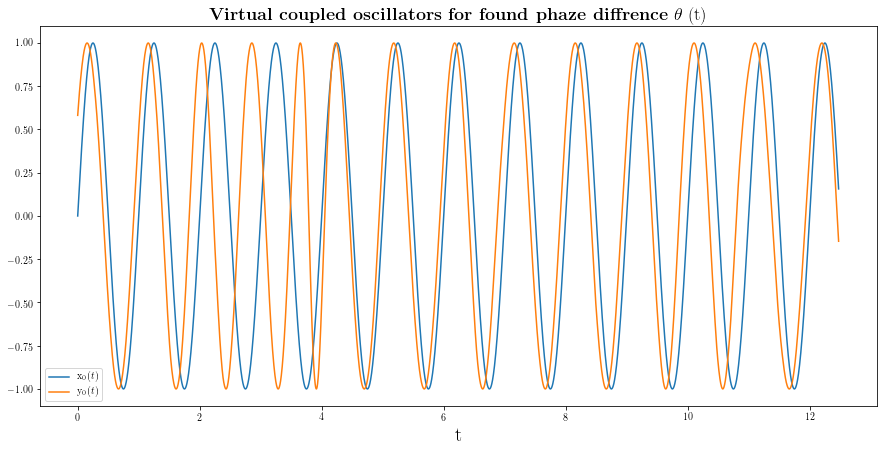
\includegraphics[width=0.7\textwidth]{stk2-3.png}
\end{center}
\end{frame}

\end{document}